\documentclass[10pt,handout]{beamer}
\usepackage{../../ikany}

\usepackage[small]{eulervm}
\usefonttheme{professionalfonts}
\usefonttheme[onlymath]{serif}

\title{Diachrony of Spectra}
\author{Ikhan Choi \\ \quad \\ Postech - Unist - Kaist Joint Seminar}

\begin{document}
\maketitle

\begin{frame}
\frametitle{Introduction}
  \pause
  \begin{defn}
    Let $R$ be a commutative ring.
    The \emph{spectrum} of $R$ is the set of prime ideals of $R$.
  \end{defn}
  \pause
  \begin{ex}
  	\[\Spec(\Z)=\{\{0\},\,2\Z,3\Z,5\Z,7\Z,11\Z,\cdots\,\}.\]
  \end{ex}
  \pause
  \begin{qn}
    Why is it defined like this?
  \end{qn}
\end{frame}


\section{Hydrogen atom}
\begin{frame}
\frametitle{Contents}
  \tableofcontents[currentsection]
\end{frame}

\begin{frame}
\frametitle{Hydrogen spectral series}
  \begin{figure}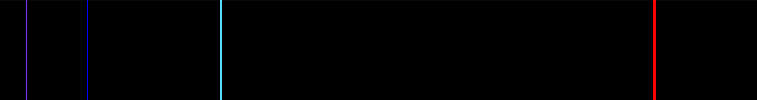
\includegraphics[scale=.4]{emission.png}\end{figure}
  \pause 410.2nm \hspace{3em} 468.1nm \hspace{13em} 656.3 nm\\ \hspace{2em} 434.0nm\\
  \bigskip
  \pause
  \begin{qn}
    How can we explain and compute this phenomenon?
  \end{qn}
  \pause \textbf{A:} By the following formula!
  \[\frac1\lambda=R\left(\frac1{n_1^2}-\frac1{n_2^2}\right),\quad\text{for}\quad n_1,n_2\in\N.\]
\end{frame}

\begin{frame}
\frametitle{Rydberg's formula (1): Bohr model}
  Bohr's postulates:\pause
  \begin{itemize}[<+->]
    \item The electrons are on certian stable orbits.
    \item The stationary orbits are computed by the old quantization assumption for angular momenta:
    \[mvr=n\hslash.\]
    \item An electron absorbs or emits light frequency $f$ when they jump from an orbit to another, satisfying
    \[\Delta E=hf.\]
  \end{itemize}
  \uncover<5->{The constant $h$ is called the Planck constant and $\hslash:=\frac h{2\pi}$.}
\end{frame}

\begin{frame}
\frametitle{Rydberg's formula (1): Bohr model}
  From the three relations
  \[mvr=n\hslash,\quad\frac{mv^2}r=-k\frac{(+e)(-e)}{r^2},\quad E=K+V=\frac12mv^2-k\frac{e^2}r,\]
  \pause we deduce
  \[E=-\frac{k^2e^4m}{2\hslash^2}\frac1{n^2}\approx-13.6\frac1{n^2}\ (eV).\]
  \pause
  \begin{prop}[Rydberg formula]
    The wavelengths $\lambda$ of absorbed or emitted photons from a hydrogen atom is estimated by the following formula:
    \[\frac1\lambda=R\left(\frac1{n_1^2}-\frac1{n_2^2}\right),\quad\text{for}\quad n_1,n_2\in\N,\]
    where $R:=\frac{k^2e^4m}{4\pi\hslash^3c}$ is the \emph{Rydberg constant}.
  \end{prop}
\end{frame}

\begin{frame}
\frametitle{Rydberg's formula (2): Schr\"odinger equation}
  More mathematically!\\
  \pause In quantum mechanics, an electron around a hydrogen atom is described by the Schr\"odinger equation: for $(t,x)\in\R^{1+3}$
  \[i\hslash\pd{t}\Psi(t,x)=-\frac{\hslash^2}{2m}\del^2\Psi(t,x)+V(x)\Psi(t,x),\]
  \pause \hspace{6em} energy \hspace{2em} kinetic energy \hspace{1em} potential energy\\
  \bigskip
  \pause where $V$ is given by the Coulomb potential
  \[V(x)=-k\frac{e^2}{|x|}.\]
  \pause By solving it, we obtain the probability distribution $|\Psi(t,x)|^2$ of the electron at time $t$, hence the assumption $\forall t,\ \int|\Psi(t,x)|^2\,dx=1<\infty$.\\
  \pause Let's solve.
\end{frame}

\begin{frame}
\frametitle{Separation of variables and Eigenvalue problems}
  \[i\hslash\pd{\Psi(t,x)}{t}=-\frac{\hslash^2}{2m}\del^2\Psi(t,x)+V(x)\Psi(t,x).\]
  \pause ``Mathematization'':
  \[i\pd_t\Psi(t,x)=(-\Delta+V(x))\Psi(t,x),\qquad V(x)=-\frac2{|x|}.\]
  \pause \textbf{Ansatz:} if the solutions has the form $\Psi(t,x)=\phi(t)\psi(x)$, \pause then
  \[\frac{i\pd_t\phi(t)}{\phi(t)}=\frac{(-\Delta+V(x))\psi(x)}{\psi(x)}\pause=E\]
  for some constant $E$, which is interpreted as the energy of electron.\\
  \pause $\therefore$ We have two \emph{eigenvalue problems} with \emph{shared eigenvalue} $E$:
  \[i\dd{t}\phi(t)=E\phi(t),\qquad(-\Delta+V(x))\psi(x)=E\psi(x).\]
  (Solutions may or may not exist according to $E$!)
\end{frame}

\begin{frame}
\frametitle{Separation of variables and Eigenvalue problems}
  Suppose we already have found the solutions $\phi_E(t)$, $\psi_E(x)$ of the eigenvalue problems for each complex number $E$.\\
  Here are some facts:
  \pause
  \begin{itemize}[<+->]
    \item Functions of the form $\Psi(t,x)=\phi_E(t)\psi_E(x)$ and linear combinations of them are solutions of the original Schr\"odinger equation.
    \item It is known that \emph{all solutions are found in this way}: general solution of the original Schr\"odinger equation is given by
    \[\Psi(t,x)=\sum_E\phi_E(t)\psi_E(x)\quad\text{or}\quad\int_E\phi_E(t)\psi_E(x)\,dE.\]
    \item For a given $E$, $\phi_E$ and $\psi_E$ are of course not unique. In fact they form a vector space which is called the eigenspace.
    \item Note that for some $E$ we probably cannot find the solution $\psi_E(x)$ that satisfies $\int|\psi_E(x)|^2\,dx=1$: the eigenspace is trivial.
    \item Since $\phi_E(t)\propto e^{-iEt}$ is easily solved, the main difficulty is $\psi_E$.
  \end{itemize}
\end{frame}

\begin{frame}
\frametitle{Separation of variables and Eigenvalue problems}
  So, here are what we need to investigate seriously:
  \pause\emph{what are the eigenvalues and eigenvectors of the linear operator}
  \[\cH:L^2(\R^3)\to L^2(\R^3)\]
  \emph{defined by}
  \[\cH\psi(x):=(-\Delta-2|x|^{-1})\psi(x)?\]
  \emph{Also, how can we compute them?}
  \pause \[\star\star\star\textbf{ The Beginning of Spectral Theory }\star\star\star\]
  \pause \vspace{-2em}
  \begin{rmk}
    Simply, $L^2(\R^3)$ is the space of $f:\R^3\to\R$ such that $\int|f|^2<\infty$. In fact, there are many technical issues to formalize this problem, for example, $L^2$ function is in general not differentiable.\\
    \pause Don't be so pedantic in doing physics.
  \end{rmk}
\end{frame}

\begin{frame}
\frametitle{Eigenvalues of hydrogen Hamiltonian}
  Anyway, with long long calculations and hard hard mathematics, experts have found the following result:
  \begin{prop}
    The eigenvalues of the operator $\cH=-\Delta-2|x|^{-1}$ are \pause
    \[-1,-\frac14,-\frac19,-\frac1{16},\cdots\]
    \pause with multiplicity 1, 4, 9, 16 and so on.
  \end{prop}
  \begin{itemize}[<+->]
    \item Eigenvalues embody the possible energies of an electron, so we can give the Rydberg formula a reasonable explanation.
    \item This result explains not only the discretized energy spectrum but also the number of orbitals in each electron shell!
    \item We call the set of eigenvalues by (discrete) \textbf{spectrum} of $\cH$.
  \end{itemize}
\end{frame}

\begin{frame}
\frametitle{Eigenvalues of hydrogen Hamiltonian}
  The simultaneous equation is solved when $E=-\frac1{n^2}$ for some $n\in\N$:
  \[i\dd{t}\phi(t)=E\phi(t),\qquad(-\Delta+V(x))\psi(x)=E\psi(x).\]
  \pause General solution of the Schr\"odinger equation is like
  \begin{align*}
    \Psi(t,x)&=\sum_{n=1}^\infty\phi_n(t)\psi_n(x)\\
    &=\sum_{n=1}^\infty e^{i\frac1{n^2}t}\left(\sum_{i=1}^{n^2}c_{n,i}\psi_{n,i}(x)\right)\\
    &=\sum_{n=1}^\infty e^{i\frac1{n^2}t}\sum_{l=0}^{n-1}\sum_{m=-l}^lc_{nlm}\ \psi_{nlm}(x).
  \end{align*}
\end{frame}

\begin{frame}
\frametitle{Conclusion of Section 1}
  \begin{rd}
  Partial Differential Equations with Time Evolution \ar{d}{Separation of variables}\\
  Simultaneous Eigenvalue Problems \ar{d} \\
  Study of Eigenvalues $=$ Study of Hydrogen Spectrum
  \end{rd}
\end{frame}


\section{Spectral theory on Hilbert spaces}
\begin{frame}
\frametitle{Contents}
  \tableofcontents[currentsection]
\end{frame}

\begin{frame}
\frametitle{Spectral theory?}
  So far, we have seen that spectral theory refers to the theory about eigenvalues and eigenvectors, \pause especially often for INFINITE dimensional linear operators.\\
  \pause In this section, we
  \begin{itemize}
    \item review the spectral theory on finite dimensional vector spaces,
    \item introduce Hilbert spaces --- a typical example of infinite dimensional vector spaces --- to state some results which extend the spectral theory to infinite dimensional spaces,
    \item and give a precise definition of ``spectrum'' of an operator.
  \end{itemize}
  \pause From now, we basically assume the scalar field as $\C$.
\end{frame}

\begin{frame}
\frametitle{Spectral theorem for matrices}
  The term ``spectral theorem'' is given to several theorems that show a condition for a linear operator to be diagonalizable.\\
  (diagonalizability is the firstly considered ``spectral property''!)\\
  \pause In particular, spectral theorems state the relation
  \[\text{condition related to adjoint} \iff \text{a kind of diagonalizability}.\]
  \pause \vspace{-1em}
  \[\begin{array}{c}\text{Vector space}\\\text{with inner product}\end{array}\hspace{4em}\begin{array}{c}\text{Vector space}\\without\ \text{additional structure}\end{array}\]
  \pause The most famous examples are for:
  \begin{defn}
    Let $V$ be a finite dimensional complex inner product space and $A:V\to V$ be linear.
    (i.e., let $A$ be a complex square matrix.)
    Then, $A$ is said to be \emph{normal} if $AA^*=A^*A$, and \emph{Hermitian} if $A=A^*$
  \end{defn}
  \pause Note that the conjugate transpose depends on the inner product structure: $A^*$ is defined by
  \[\<x,Ay\>=\<A^*x,y\>.\]
\end{frame}

\begin{frame}
\frametitle{Spectral theorem of matrices}
  \begin{thm}[Spectral theorem for normal matrices]
    A complex square matrix $A$ is normal if unitarily diagonalizable.
  \end{thm}
  \begin{thm}[Spectral theorem for Hermitian matrices]
    A complex square matrix $A$ is Hermitian if unitarily diagonalizable and all eigenvalues are real.
  \end{thm}
  \bigskip
  \pause TFAE: a matrix is/has
  \begin{itemize}
    \item unitarily diagonalizable
    \item a set of eigenvectors forms an orthonormal basis of $V$.
  \end{itemize}
  \pause Remind what we did in the previous section.
  The purpose of separation of variables is to \emph{construct an orthonormlal basis for the solution space.}
\end{frame}

\begin{frame}
\frametitle{Hilbert space}
  \pause
  \begin{defn}
    An inner product space, possibly infinite dimensional, is called a \emph{Hilbert space} if it is complete; the metric
    \[d(x,y):=\sqrt{\<x-y,x-y\>}\]
    has the space become a complete metric space.
  \end{defn}
  \pause
  \begin{itemize}[<+->]
    \item The vector space $C^n$ $\iff$ Finite dimensional Hilbert space.
    \item The space $L^2(X)$ is a Hilbert space with $\<f,g\>:=\int_X fg\,dx$.
    \item Conversly, Hilbert space usually means the $L^2$ space of wave functions, by physicists.
    \item The space $\ell^2(\C)$ of sqare summable sequeces is a Hilbert space with $\<(a_n),(b_n)\>:=\sum_na_nb_n$.
  \end{itemize}
\end{frame}

\begin{frame}
\frametitle{Bounded operators}
  \begin{thm}[?]
    In finite dimensions, something linear is always continuous.
  \end{thm}
  \pause \begin{itemize} \item However, this may be wrong in infinite dimensions.\\ We should find linear operators of nicer properties to state the generalized spectral theorem.\end{itemize} \pause
  \begin{defn}
    A linear operator $T:H\to H$ on a Hilbert space is called \emph{bounded} if there is a constant $C>0$ such that for all $x\in H$
    \[\|Ax\|\le C\|x\|.\]
    The set of bounded operators on $H$ is denoted by $B(H)$.
  \end{defn}
  \pause
  \begin{thm}
    A linear operator on a Hilbert space is bounded iff continuous.
  \end{thm}
\end{frame}

\begin{frame}
\frametitle{Compact operators}
  Bounded operators are not enough.
  \begin{defn}
    A linear operator $T$ on a Hilbert space is called \emph{compact} if image of bounded set is relatively compact.
  \end{defn}
  \pause
  \begin{rmk}
    The closed ball in infinite dimensional Hilbert space is not compact: we can find a sequence not having any convergent subsequence.
  \end{rmk}
  \pause
  \begin{ex}
    An operator $T:\ell^2\to\ell^2$ defined by
    \[T(a_1,a_2,a_3,\cdots)=(a_1,\frac{a_2}2,\frac{a_3}3,\cdots)\]
    is compact, but the identity $I\to\ell^2\to\ell^2$
    \[I(a_1,a_2,a_3,\cdots)=(a_1,a_2,a_3,\cdots),\]
    which is clearly bounded, is not compact.
  \end{ex}
\end{frame}

\begin{frame}
\frametitle{Spectral theorem for compact normal operators}
  \begin{thm}[Spectral theorem for compact normal operators]
    Let $T$ be a compact normal operator on a separable Hilbert space. Then, there exists a countable orthonormal basis consisting of eigenvectors, with corresponding eigenvalues that converges to 0.
  \end{thm}
  \begin{thm}[Spectral theorem for compact self-adjoint operators]
    Let $T$ be a compact self-adjoint operator on a separable Hilbert space. Then, there exists a countable orthonormal basis consisting of eigenvectors, with corresponding eigenvalues that are reals and converges to 0.
  \end{thm}
  \pause
  \begin{rmk}
    There are some concepts we will skip:
    \begin{itemize}
      \item we did not define ``separable'' space,
      \item we did not define ``countable (Schauder) basis''.
    \end{itemize}
  \end{rmk}
\end{frame}

\begin{frame}
\frametitle{Discrete spectrum}
  An application of spectral theorem:\\
  The Hamiltonian operator for harmonic oscillator $-\Delta+|x|^2$ is an example of what we call \emph{elliptic operators} with discrete spectrum.\\
  We will not deal with this in detail, but:
  \bigskip
  \begin{center}
    \pause The operator $-\Delta+|x|^2$ is unbounded,\\$\ $\\
    \pause but it is known that we can view it as the\\
    inverse of a compact self-adjoint(positive) operator.\\
    \pause $\downarrow$ \\
    The eigenvalues are distributed like
    \[0<\lambda_1<\lambda_2<\cdots\to\infty.\]
  \end{center}
  \pause Hydrogen atom is more complicated: it has both discrete spectra $\{-\frac1{n^2}\}$ and continuous spectra $[0,\infty)$.
  What is continuous spectrum?
\end{frame}

\begin{frame}
\frametitle{Continuous spectrum}
  For hydrogen atom $\impl$ we defined the discrete spectrum of Hamiltonian $\cH=-\Delta+2|x|^{-1}$ as the set of \emph{eigenvalues}.\\
  \bigskip
  \pause For a free particle $\impl$\pause$\cH=-\Delta+V=-\Delta$, we cannot; eigenvectors exist for $E\ge0$, and they are ``linear combinations'' of
  \[\psi_E(x)=e^{ik\cdot x},\qquad\text{ for }k\in\R^3\text{ s.t. }|k|^2=E,\]
  which are all not in $L^2$.\\
  \bigskip
  \pause However, their integral may serve as a solution:
  \[\Psi(t,x)=\int_Ee^{-iEt}\int_{|k|=\sqrt E}a_E(k)e^{ik\cdot x}\,dk\,dE.\]
  \pause
  \begin{itemize}
    \item Energy spectrum of free particle is not \emph{quantized} $=$ \emph{discretized}.
    \item We want to say $-\Delta$ has the spectrum $[0,\infty)$.
  \end{itemize}
\end{frame}

\begin{frame}
\frametitle{Continuous spectrum}
  \begin{defn}
    Let $T$ be an operator on a Hilbert space $H$.
    The \emph{spectrum} of $T$ is defined by
    \[\sigma(T):=\{\lambda\in\C:T-\lambda I\text{ is not invertible in }B(H)\}.\]
  \end{defn}
  \pause In particular,
  \begin{defn}
    The \emph{point spectrum} of $T$ is defined by the set of eigenvalues:
    \[\sigma_p(T):=\{\lambda\in\C:T-\lambda I\text{ is not injective }\}.\]
  \end{defn}
  \vspace{-1em}
  \begin{defn}
    The \emph{continuous spectrum} of $T$ is defined by
    \[\sigma_c(T):=\{\lambda\in\C:T-\lambda I\text{ is injective but has proper dense image }\}.\]
  \end{defn}
\end{frame}

\begin{frame}
\frametitle{Conclusion of Section 2}
  \begin{itemize}
    \item In infinite dimensional spaces, the spectral theorems are generalized for compact operators.
    \item The spectrum of an operator $T$ is defined by
    \[\{\lambda\in\C:T-\lambda I\text{ is not invertiable }\}.\]
  \end{itemize}
\end{frame}


\section{Gelfand theory}
\begin{frame}
\frametitle{Contents}
  \tableofcontents[currentsection]
\end{frame}

\newtheorem{pdefn}{Psudo-definition}
\begin{frame}
\frametitle{$C^*$-algebras}
  The goal of this section is to state the Gelfand-Naimark theorem, which crucially affects to the definition of $\Spec(R)$.
  \pause We give definitions:
  \begin{pdefn}
    An \emph{algebra} is a vector space with vector multiplication.\\
    Equivalently, a ring with scalar multiplication.
  \end{pdefn}
  \pause
  \begin{defn}
    A \emph{$C^*$-algebra} is a complex associative algebra with involution $*$ and norm $\|\cdot\|$ such that the norm is complete and $\|x^*x\|=\|x^*\|\|x\|$.
  \end{defn}
  \pause
  \begin{ex}[1]
    Let $H$ be a complex Hilbert space.
    Then, $B(H)$ is a $C^*$-algebra.
    $C^*$-algerbras are invented to learn the abstract study of $B(H)$.
  \end{ex}
  \pause
  \begin{ex}[2]
    Let $X$ be a compact space.
    Then, the set of complex-valued continuous functions $C(X,\C)$ is a commutative $C^*$-algebra.
  \end{ex}
\end{frame}

\begin{frame}
\frametitle{Gelfand theory (1): continuous function space}
  Assumption: unless mentioned otherwise, we will only discuss \emph{commutative unital} $C^*$-algebras.\\
  \smallskip\pause The following definition is natural:
  \begin{defn}
    Let $A$ be (possibly non-commutative) $C^*$-algebra.
    A complex number $\lambda$ is in the \emph{spectrum} of $a\in A$ if $a-\lambda e$ is not invertible.
    The spectrum is denoted by $\sigma(a)$.
  \end{defn}
  \bigskip\pause
  What can be told for a continuous function on a compact $X$? For $C(X)$,\pause
  \begin{itemize}[<+->]
    \item $\sigma(f)=\im(f)$,
    \item every maximal ideal is of the form $\{f:f(x)=0\}$ for a single point $x\in X$.
  \end{itemize}
\end{frame}

\begin{frame}
\frametitle{Gelfand theory (2): generated $C^*$-subalgebra}
  The following is also an important exmple to formulate functional calculus:
  \begin{defn}
    Let $A$ be a (possibly non-commutative) $C^*$-algebra.
    An element $a\in A$ is called \emph{normal} if $a^*a=aa^*$.
    For a normal element, a $C^*$-subalgebra defined by
    \[C^*(a):=\cl{\{\,p(a,a^*):p\in\C[x,y]\,\}}\subset A\]
    is said to be \emph{generated by} $a$.
  \end{defn}
  \pause Note that $C^*(a)$ is commutative since $a$ is normal! For $C^*(a)$,
  \pause
  \begin{itemize}[<+->]
    \item if $a-\lambda$ is not invertible, there we can assign a maximal ideal containing it,
    \item conversely, for a maximal ideal $\fm$, the image of $a$ under the projection $C^*(a)\to C^*(a)/\fm\cong\C$ is in a spectrum of $a\ ^{(*)}$,
    \item the maps above are inverses of each other.
  \end{itemize}
  \uncover<5->{Therefore,}
\end{frame}

\begin{frame}
\frametitle{Gelfand theory (2): generated $C^*$-subalgebra}
  \begin{prop}
    There is a 1-1 correspondence between
    \[\text{spectrum of $a$}\iff\text{maximal ideal space of $C^*(a)$}.\]
  \end{prop}
  \pause
  Consider $C(X)$.
  The above proposition states that image is corresponded to its domain: the element $a$ acts like an ``injective function'' in $C^*(a)$.
  \pause
  \begin{defn}
    Let us define the \emph{spectrum} of general commutative unital $C^*$-algebra $A$ as the \textbf{set of maximal ideals} and denote it by $\sigma(A)$.
  \end{defn}
\end{frame}

\begin{frame}
\frametitle{Spectrum as a topological space}
  Let $\sigma(A)$ be the spectrum of a comm. unit. $C^*$-algebra $A$.\\
  \smallskip
  \pause We set up the \emph{topology of pointwise convergence} on $\sigma(A)$, by identifying maximal ideals with the projections to $\C$:\\
  \smallskip
  for example, consider $C(X)$.
  Since $X$ is naturally 1-1 corresponded to $\sigma(C(X))$ as a set,
  \[x\to y\in X \iff f(x)\to f(y)\quad\text{ for all }f\in C(X).\]
  \pause
  Then,
  \begin{prop}
    Let $A$ be a comm. unit. $C^*$-algebra.
    Then, the spectrum $\sigma(A)$ is compact (by the Banach-Alaoglu).
  \end{prop}
  \pause
  \begin{ex}
    For the space $\ell^1$ of summable sequences, the spectrum is the unit circle: $\sigma(\ell^1)=\T$.
  \end{ex}
  \begin{ex}
    Let $X$ be compact Hausdorff. Then, $\sigma(C(X))$ is homeomorphic to $X$.
  \end{ex}
\end{frame}

\begin{frame}
\frametitle{Gelfand-Naimark theorem}
  Finally, we state the Gelfand-Naimark theorem. \pause
  \begin{thm}[Gelfand-Naimark, 1943]
    Let $A$ be a commutative unital $C^*$-algebra.
    Then, we have a $C^*$-algebra isomorphism
    \[A\to C(\sigma(A)).\]
    This map is called \emph{Gelfand representation}.
  \end{thm}
\end{frame}

\begin{frame}
\frametitle{Conclusion of Section 3}
  Transitions of definition:
  \begin{itemize}
    \item Spectrum of $a\in A$ $\to$ generalized eigenvalues;
    \item Spectrum of $a\in C(X)$ $\to$ image of function;
    \item Spectrum of $a\in C^*(a)$ $\to$ maximal ideals;
  \end{itemize}
  \hspace{10em}$\Downarrow$
  \begin{itemize}
    \item Spectrum of $C(X)$ $:=$ maximal ideals $=$ domain $=$ image of inj,\\
    \item Spectrum of $A$ $:=$ maximal ideals ($\approx$ domain(?)).
  \end{itemize}
  \bigskip
  \[\text{Spectrum}\iff\{\text{Maximal ideals}\}\iff\{\text{Points}\}\]
\end{frame}


\section{Algebraic geometry}
\begin{frame}
\frametitle{Contents}
  \tableofcontents[currentsection]
\end{frame}

\begin{frame}
\frametitle{Algebraic geometry}
  In algebriac geometry, we...
  \begin{itemize}
    \pause\item Want to describe geometry with polynomials:\\
      \quad The circle is described by the polynomial $x^2+y^2-1$.
    \pause\item Want to solve geometric problems with properties of polynomials:\\
      for example,
      \begin{itemize}
        \item to compute the number of singularity,
        \item to determine the topological shape,
        \item to investigate the dimension of intersection, etc.
      \end{itemize}
    \pause\item Want to make a correspondence between geometry and algebra:\\
      ($\to$) use algebraic computations to analyze geometry,\\
      ($\leftarrow$) use the geometric intuition to study algebra.
  \end{itemize}
  \pause In this section, assume that a ``ring'' is a commutative and unital one.
\end{frame}

\begin{frame}
\frametitle{Algebraic variety}
  \begin{rmk}
  We give basic definitions here.
  For simplicity, we will do everything in the three dimension $\C^3$.
  Every concept is directly generalized to arbitrary dimensions.
  \end{rmk}
  \pause
  \begin{defn}
    Let $T\subset\C[x,y,z]$ and define
    \[\cZ(T):=\{p\in\C^3:f(p)=0\text{ for all }f\in T\}.\]
    An \emph{algebraic set} is a subset $V$ of $\C^n$ satisfying $V=Z(T)$ for some $T$.
  \end{defn}
  \pause
  \begin{defn}
    Let $Y\subset\C^n$ and define
    \[\cI(Y):=\{f\in\C[x,y,z]:f(p)=0\text{ for all }p\in Y\}.\]
    This is always a radical(square-free) ideal.
  \end{defn}
\end{frame}

\begin{frame}
\frametitle{Algebraic variety}
  \begin{prop}\begin{itemize}
    \item For an algebraic set $V\subset\C^3$, we have $\cV(\cI(V))=V$.
    \item For a radical ideal $I\subset\C[x,y,z]$, we have $\cI(\cV(I))=I$.
  \end{itemize}\end{prop}
  \pause
  \begin{defn}
    If an algebraic set is not a union of two proper algebraic subsets, then it is called \emph{algebraic variety}.
  \end{defn}
  \begin{prop}
    An algebraic set $V$ is an algebraic variety iff $\cI(V)$ is prime.
  \end{prop}
  \pause
  \[\text{algebraic sets}\iff\text{radical ideals},\]\vspace{-1em}
  \[\text{algebraic varieties}\iff\text{prime ideals}.\]
\end{frame}

\begin{frame}
\frametitle{Coordinate ring}
  Consider an algebraic variety $S^2=\{x^2+y^2+z^2=1\}$.
  The following two functions are same on $S^2$:
  \[f=x+1,\qquad g=x+x^2+y^2+z^2.\]
  In other words, $f-g\in\cI(S^2)$.
  \pause
  \begin{defn}
    A \emph{coordinate ring} or \emph{structure ring} of an algebraic set $V$ is the ring $\C[x,y,z]/\cI(V)$.
  \end{defn}
  \bigskip
  Every ring of the form $\C[x,y,z]/I$, where $I$ is an ideal, we can interpret the ring as the set of functions on the algebraic set $\cV(I)$.
  Why do we introduce this?\\
  \smallskip
  \pause \textbf{Main Philosophy of AG}:\\
  \qquad\qquad analyze the \emph{function space} to study geometric objects!
\end{frame}

\begin{frame}
\frametitle{Krull dimension}
  Let us see an example that shows the power of structure rings.
  \begin{center}
  \begin{tabular}{lcl}
  Equation & Ideal & Dimension \\ \hline
  $\mt$ & $\mt$ & 3 \\
  $x=1$ & $(x-1)$ & 2 (plane)\\
  $x=1$, $y=2$ & $(x-1,y-2)$ & 1 (line)\\
  $x=1$, $y=2$, $z=3$, & $(x-1,y-2,z-3)$ & 0 (point)
  \end{tabular}
  \end{center}
  \pause
  Coordinate rings are
  \begin{gather*}
    \C[x,y,z],\ \C[x,y,z]/(x-1),\\
    \C[x,y,z]/(x-1,y-2),\ \C[x,y,z]/(x-1,y-2,z-3).
  \end{gather*}
  \begin{defn}
    The \emph{Krull dimension} of a ring $R$ is the maximal length of chain of prime ideals.
  \end{defn}
  $\therefore$ The Krull dimension of coordinate ring is same with the ``dimension'' of the corresponding algebraic sets.
\end{frame}

\begin{frame}
\frametitle{Maximal ideal is a point}
  Second example.
  \begin{thm}
  The ideal $(x-a,y-b,z-c)$ is maximal in $\C[x,y,z]$.
  \end{thm}
  \pause Conversely,
  \begin{thm}[Weak Hilbert Nullstellensatz]
    Every maximal ideal in $\C[x,y,z]$ has the form
    \[(x-a,y-b,z-c).\]
  \end{thm}
  \pause This theorem implies that we have the following correspondence:
  \[\text{points}\iff\text{maximal ideals}.\]
\end{frame}

\begin{frame}
\frametitle{Alexander Grothendieck}
  \begin{figure}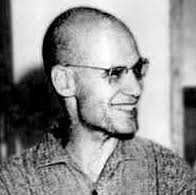
\includegraphics[scale=.4]{grothendieck.jpeg}\end{figure}
  \begin{center}
  Alexander Grothendieck (1928 - 2014)\\
  \uncover<4>{\emph{original major: functional analysis!!!}}\\
  ``Every ring should be recognized as the set of functions on a space.''\\
  \end{center}
  \pause What space? \pause Spectrum!
\end{frame}

\begin{frame}
\frametitle{Problems of maximal ideals}
  First trial:
  \begin{defn}
    Let $R$ be a ring.
    Define the \emph{spectrum} of $R$ as the set of maximal ideals.
  \end{defn}
  \bigskip
  \pause But it had two problems:
  \begin{enumerate}
    \item The codomain is not unified;
    \item We want the spectrum to have a \emph{functoriality}.
  \end{enumerate}
\end{frame}

\begin{frame}
\frametitle{Gelfand-Mazur theorem}
  Let $\fm$ be a maximal ideal($=$point) of the ring $R$.
  Then, codomian field of functions at the point is characterized by the quotient $R/\fm$.\\
  \pause For $C^*$-algebras, we could just use the maximal ideals becuase the field $R/\fm$ is always isomorphic to $\C$:
  \begin{thm}[Gelfand-Mazur]
    A $C^*$-algebra that is a field, is isormophic to $\C$.
  \end{thm}
  \pause However, when we are concerned with general ring $R$, we cannot guarantee such results.\\
  There are two choices about the codomain problem:\pause
  \begin{enumerate}
    \item Restrict the condition for maximal ideals,
    \item Compromise the unifies codomain.\pause (v)
  \end{enumerate}
\end{frame}

\begin{frame}
\frametitle{Functoriality}
  We want $\Spec:\cat{CRing}\to\cat{Set}$ to be a (contravariant) functor:\\
  functoriality allows to define schemes and apply the powerful theory of sheaves to AG.
  \pause Under what definitions is a ring homomorphism $R\to S$ able to induce the map $\Spec(S)\to\Spec(R)$? \pause
  \begin{ex}
    Consider the ring homomorphism $i:\Z\emb\Q$.
    The most reasonable choice of the naturally induced map is
    \[\Spec(\Q)\to\Spec(\Z):p\mapsto i^{-1}(p).\]
    \pause If $\Spec$ is defined to be the set of maximal ideals, then the functoriality is not satisfied: $(0)$ is maximal in $\Q$, but $i^{-1}((0))=(0)$ is not maximal in $\Q$.
  \end{ex}
  \pause
  \begin{prop}
    Inverse image of prime ideal under a ring homomorphism is prime.
  \end{prop}
\end{frame}

\begin{frame}
\frametitle{Conclusion}
  When Grothendieck transplanted the idea of spectrum from functional analysis to algebraic geometry, the following definition comes up:
  \begin{defn}
    Let $R$ be a ring.
    The spectrum of $R$ is the set of prime ideals.
  \end{defn}
\end{frame}


\end{document}